%**************** BASICS OF GEOMETRY ******************
\section{Basics of Differential Geometry}
To understand the applications of Ricci Flow, we need to explore the properties of Riemannian manifolds, particularly how to define a flow on a manifold and its relation to differential equations. We will see that the Ricci Flow can be viewed as a differential equation for a family of metrics on a Riemannian manifold.


%***************** DIFFERENTIABLE MANIFOLDS ********************
\subsection{Differentiable Manifolds}
\begin{figure}
	\centering
	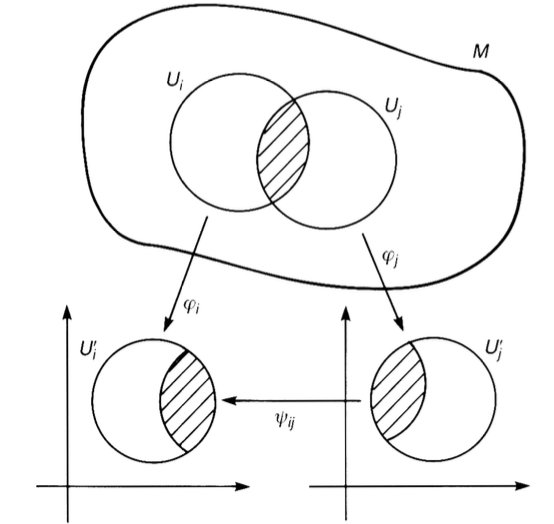
\includegraphics[width=0.5\textwidth]{Images/homeomorphism.png}
	\caption{$\phi_i$ is a homeomorphism from $U_i$ onto an open subset $U'_i$ of $\R^n$.}
	\label{fig:homeomorphism}
\end{figure}

Let's begin by defining a \emph{differentiable manifold}, ~\cite{lee:smooth,tu:manifolds}.

\begin{definition}[Differentiable manifold]
	An $n$-dimensional \emph{differentiable manifold} $\M$ is a topological space equipped with a family of pairs $\{ (U_i, \phi_i) \}$, called an \emph{atlas}, where
	\begin{itemize}
		\item Each $U_i$ is an open set in $\M$, and $\cup_i U_i = \M$.
		\item Each $\phi_i$ is a homeomorphism from $U_i$ onto an open subset $U_i'\subseteq \R^n$, as shown in fig.~\ref{fig:homeomorphism}
		\item For any $U_i$ and $U_j$ with $U_i \cap U_j \neq \emptyset$, the map
		      \begin{equation*}
			      \phi_i \circ \phi_j^{-1} \colon \phi_j (U_i \cap U_j) \to \phi_i(U_i \cap U_j),
		      \end{equation*}
		      is infinitely differentiable.
	\end{itemize}
\end{definition}

Each pair $(U_i, \phi_i)$ is called a \emph{chart}, with $U_i$ the \emph{coordinate neighbourhood} and $\phi_i$ the \emph{coordinate map}. Basically, $\phi_i$ assigns $n$ real \emph{coordinates} $\{x_1(p), \dots, x_n(p)\}$ to each point of $U_i$.

A \emph{manifold with boundary} is defined similarly, except each chart maps into the closed half-space $H^n = \{ (x^1, \dots, x^n) \in R^n | x^n \geq 0 \}$, as showed in fig.~\ref{fig:boundary}.

\begin{comment}
\begin{figure}
	\centering
	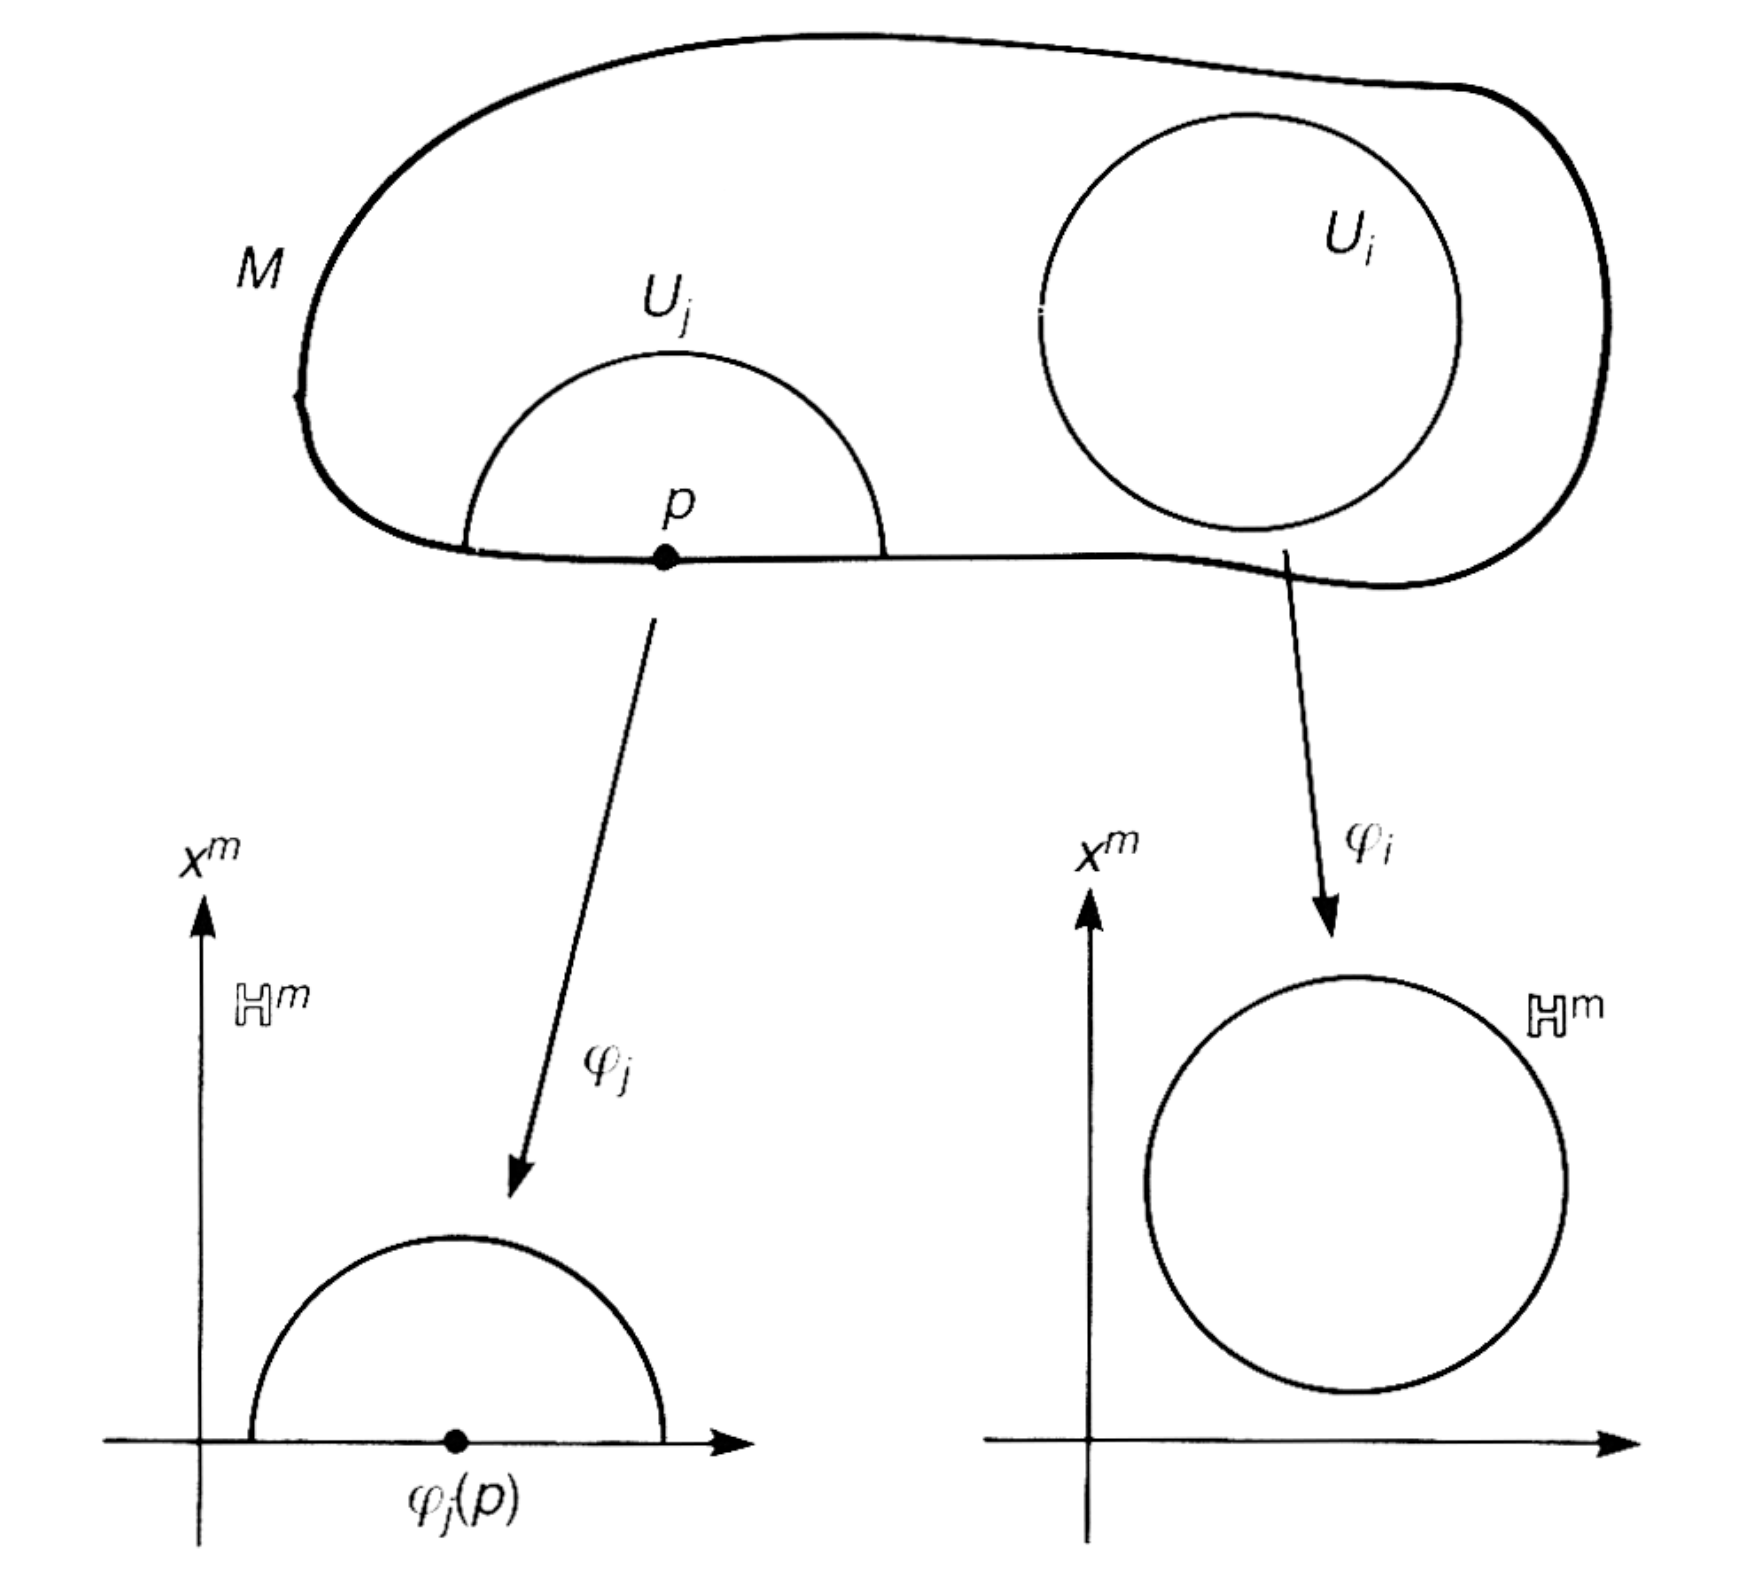
\includegraphics[width=0.5\textwidth]{Images/boundary.png}
	\caption{A manifold $\M$ with boundary. Here, $p \in \de \M$.}
	\label{fig:boundary}
\end{figure}
\end{comment}

\begin{figure}
	\centering
	\begin{subfigure}[b]{0.38\textwidth}
		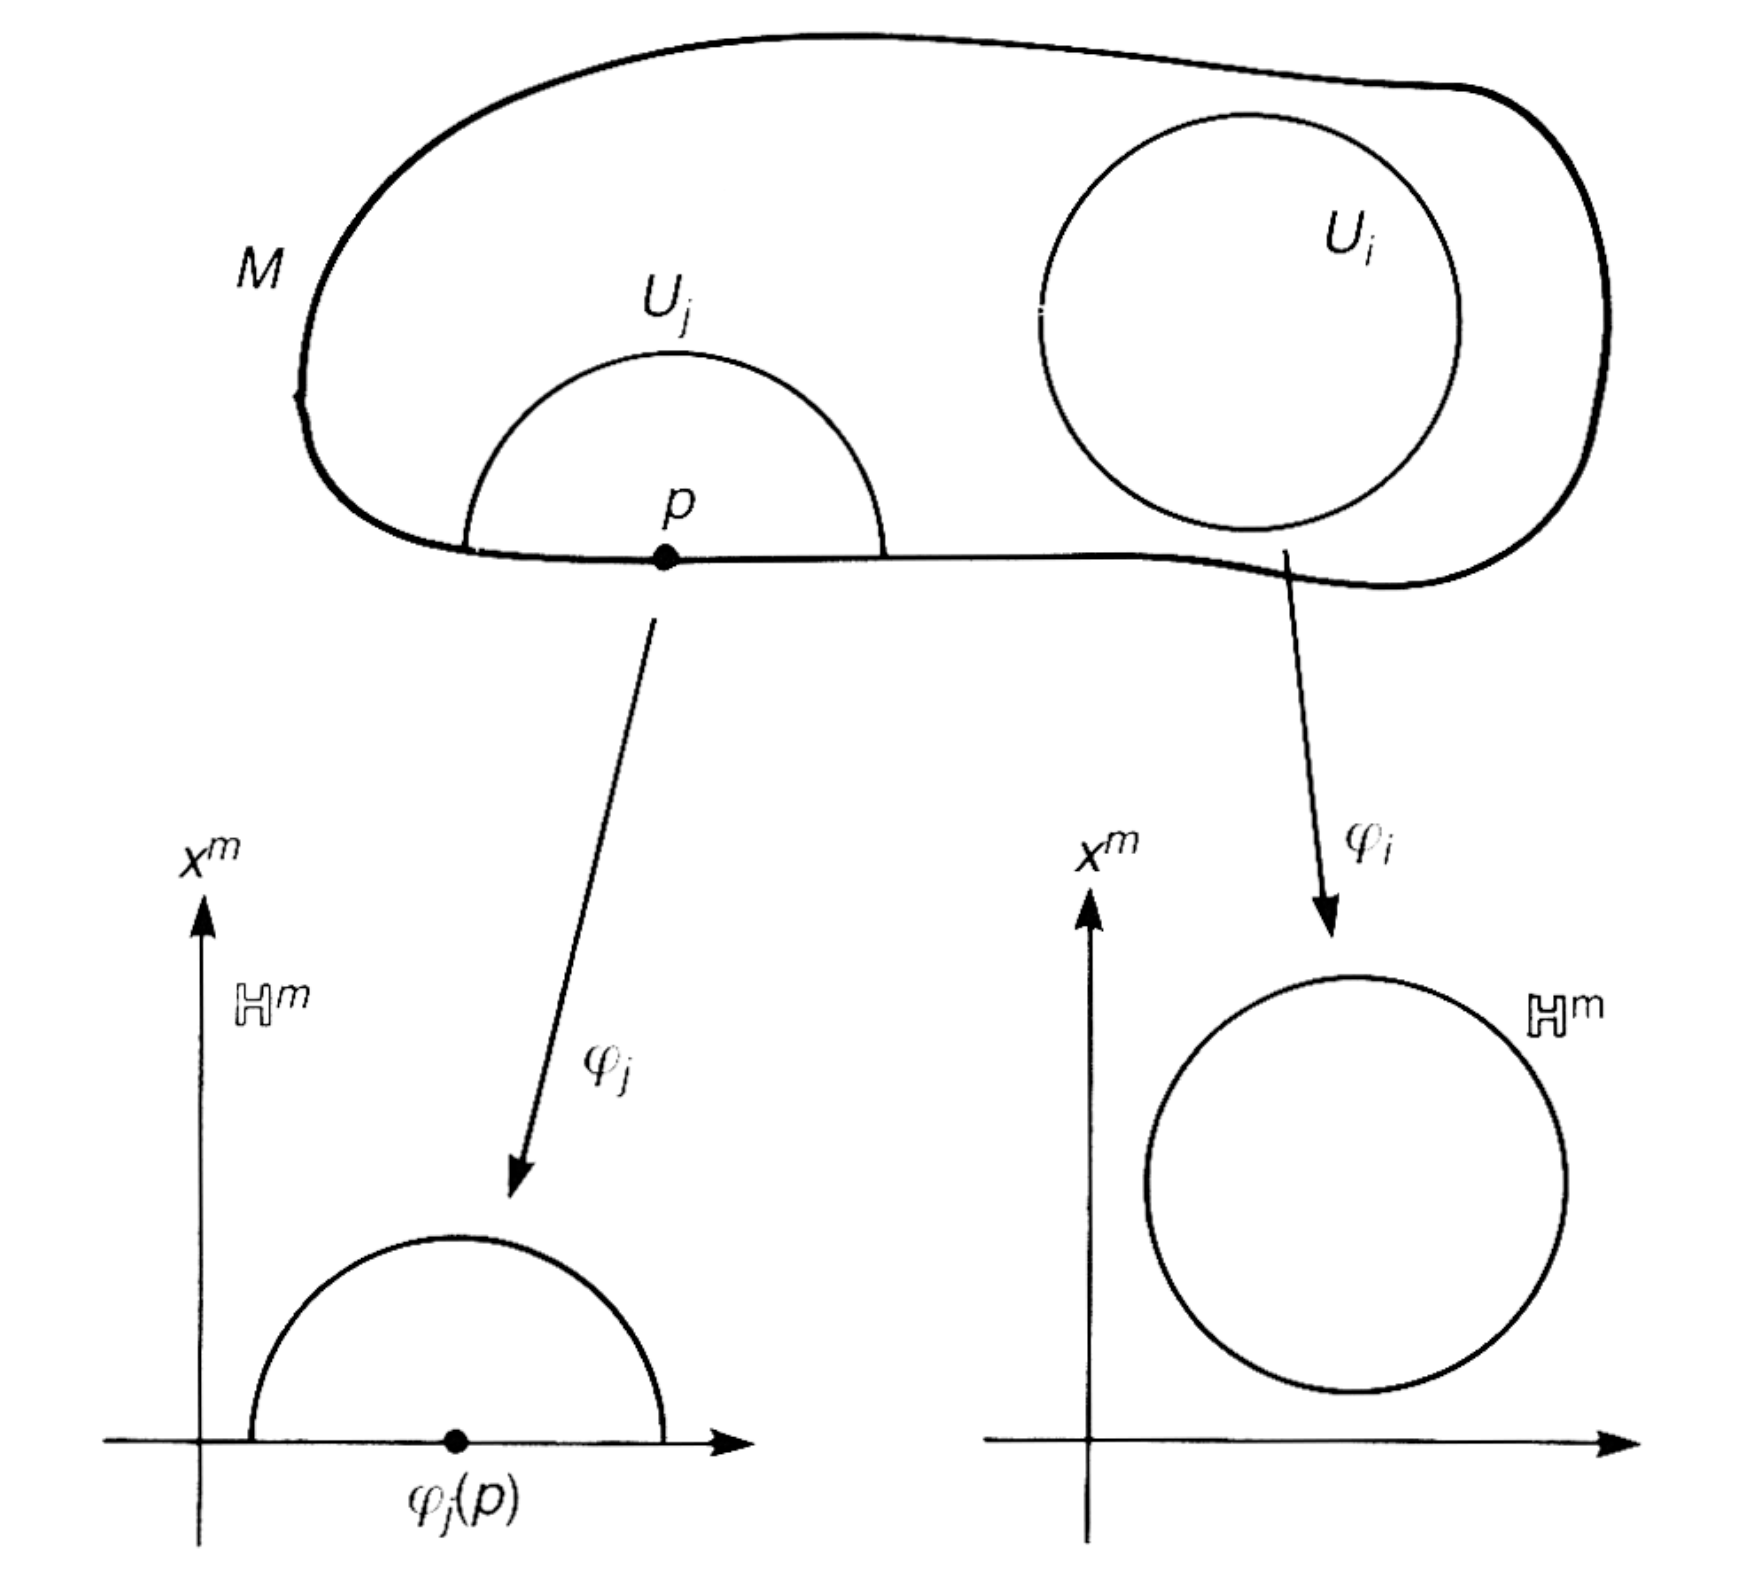
\includegraphics[width=\textwidth]{Images/boundary.png}
		\caption{A manifold $\M$ with boundary. Here, $p \in \de \M$.}
		\label{fig:boundary}
	\end{subfigure}
	\hfill
	\begin{subfigure}[b]{0.42\textwidth}
		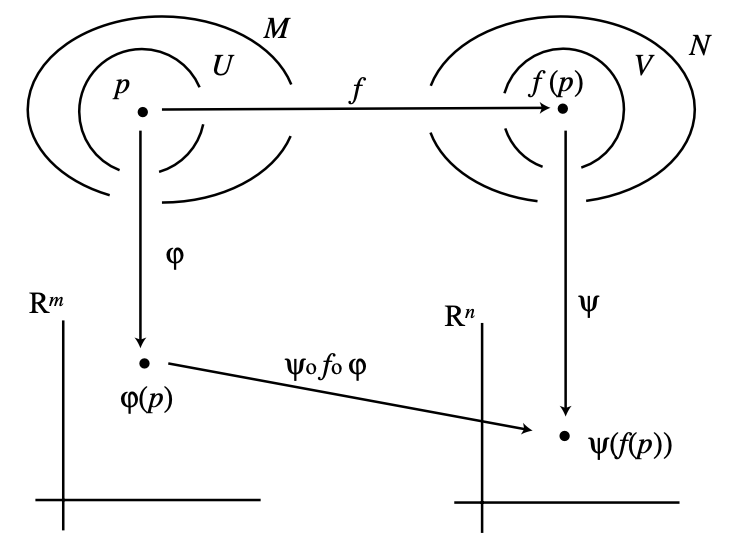
\includegraphics[width=\textwidth]{Images/map.png}
		\caption{A map $f \colon \M \to \mathcal{N}$ has coordinates representation $\psi \circ f \circ \phi^{-1} \colon \R^m \to \R^n$.}
		\label{fig:map}
	\end{subfigure}
	\caption{Manifolds with boundaries and maps.}
\end{figure}

%***************** DIFFERENTIABLE MAPS ********************
\subsection{Differentiable Maps}
Because each chart maps locally to $\R^n$, we adopt the usual notion of differentiability. Let $\M$ and $\mathcal{N} $ be manifolds of dimension $m$ and $n$, respectively. Consider a map $f: \M \to \mathcal{N}$, as shown in fig.~\ref{fig:map}. Considering the charts $(U, \phi)$ on $\M$ and $(V,\psi)$ on $\mathcal{N}$, the coordinate representation of $f$ is
\begin{equation}
	\phi \circ f \circ \phi^{-1}: \R^m \to \R^n .
\end{equation}

Relaxing the notation, we may write $\phi(p) = \{x^\mu\}$ and $\psi(f(p)) = \{y^\alpha\}$, so that $f$ is \emph{differentiable} at $p \in \M$ if $y^\alpha = f^\alpha(x^\mu)$ is.

\begin{comment}
\begin{figure}
	\centering
	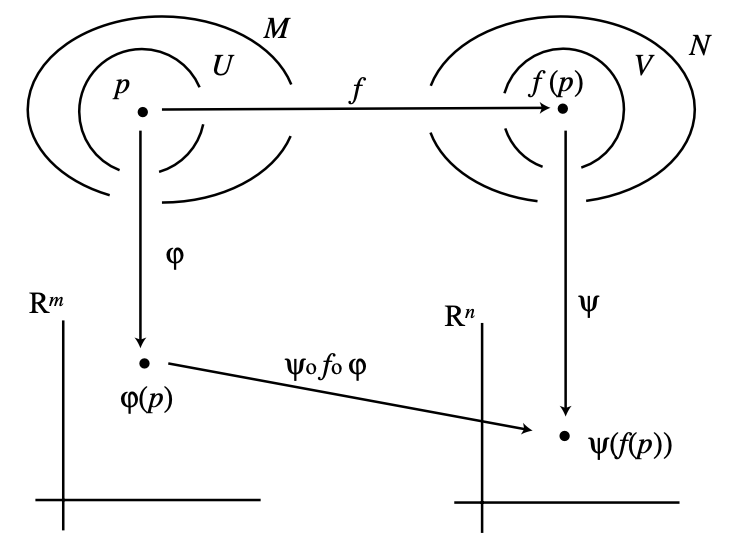
\includegraphics[width=0.5\textwidth]{Images/map.png}
	\caption{A map $f \colon \M \to \mathcal{N}$ has coordinates representation $\psi \circ f \circ \phi^{-1} \colon \R^m \to \R^n$.}
	\label{fig:map}
\end{figure}
\end{comment}

Three special classes of differentiable maps are especially relevant.

\begin{definition}[Diffeomorphism]
	Let $f \colon \M \to \mathcal{N}$ be a homeomorphism and $\psi$ and $\phi$ the same coordinate functions as before. Then, if $\psi \circ f \circ \phi^{-1}$ is invertible and both $y \equiv \psi \circ f \circ \phi^{-1}(x)$ and $x \equiv \phi \circ f^{-1} \circ \psi^{-1}(y)$ are $C^\infty$, $f$ is called a \emph{diffeomorphism} and $\M$ is said to be \emph{diffeomorphic} to $\mathcal{N}$, $\M \equiv \mathcal{N}$.
\end{definition}

\begin{definition}[Curve]
	An \emph{open curve} in an $n$-dimensional manifold $\M$ is a map $c \colon (a,b) \to \M$, where $(a,b)$ is an open interval such that $a<0<b$. A \emph{closed curve} is a map $c \colon S^1 \to \M$. On a chart $(U,\phi)$, a curve $c(t)$ has the coordinate representation $x=\phi \circ c \colon \R \to \R^n$. See fig.~\ref{fig:curve}
\end{definition}

\begin{definition}[Function]
	A \emph{function} $f$ on $\M$ is a smooth map from $\M$ to $\R$. On a chart $(U,\phi)$, the coordinate representation of $f$ is given by $f \circ \phi^{-1} \colon \R^n \to \R$, which is a real-valued function of $n$ variables. The set of functions is denoted by $\mathfrak{F}(\M)$. See fig.~\ref{fig:function}
\end{definition}

\begin{figure}
	\centering
	\begin{subfigure}[b]{0.38\textwidth}
		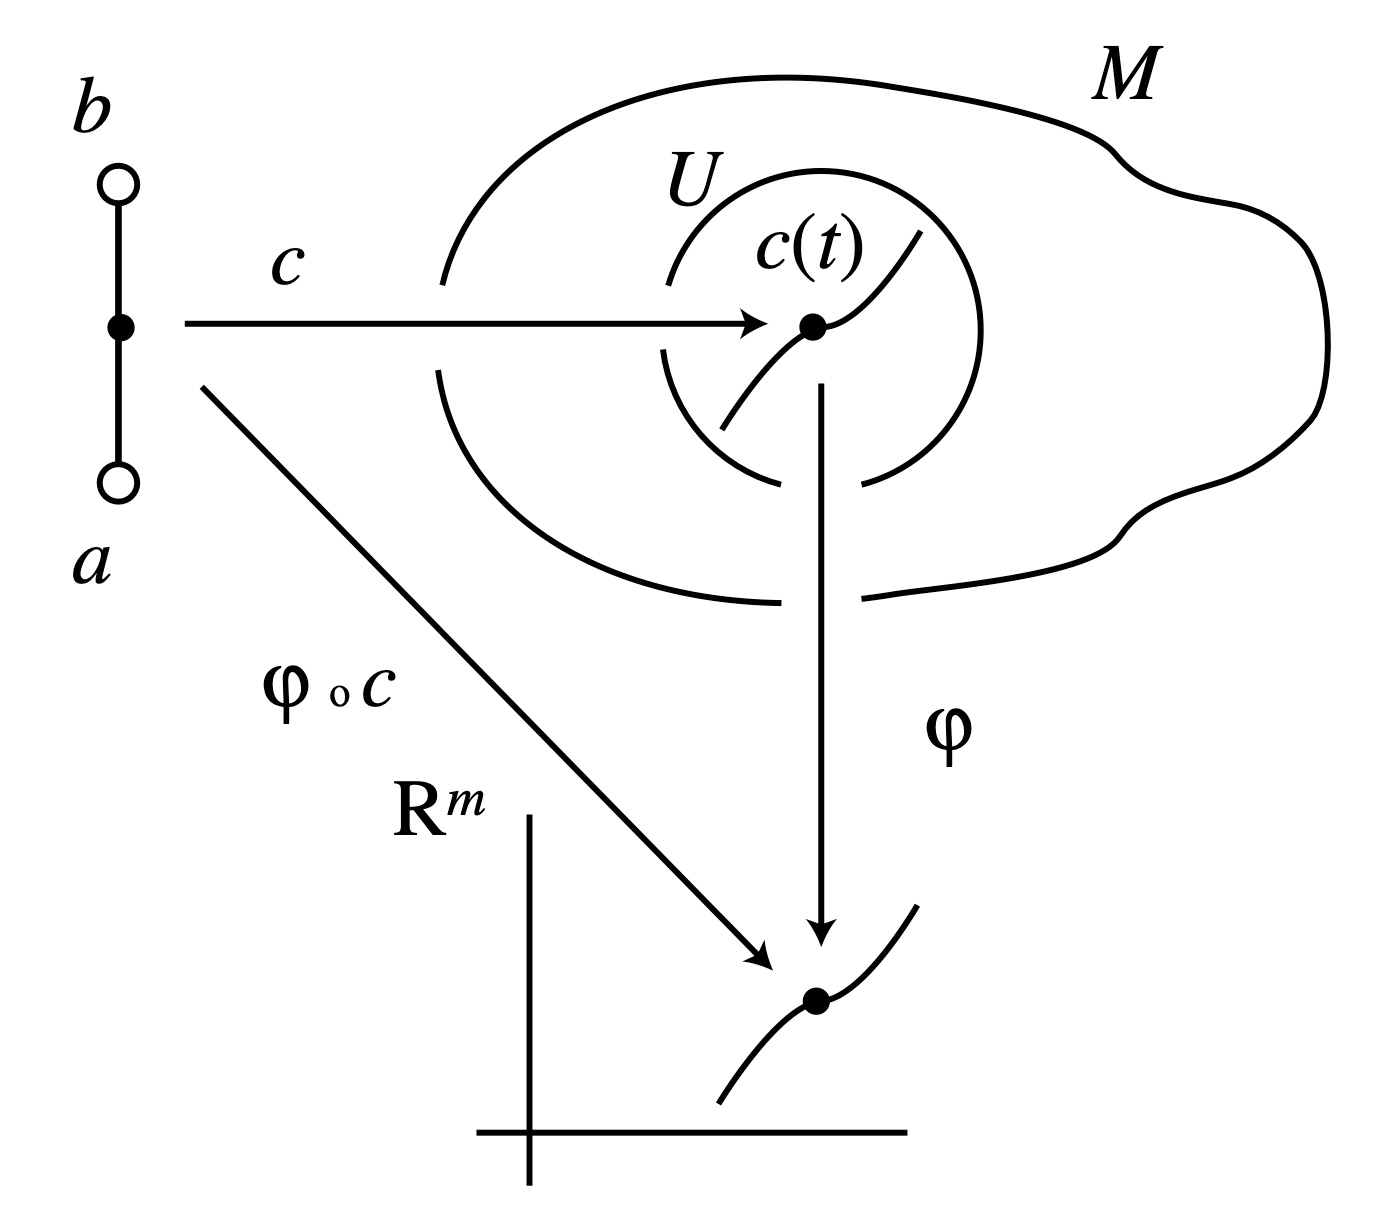
\includegraphics[width=\textwidth]{Images/curve}
		\caption{A curve $c$ in $\M$ and its coordinate representation $\psi \circ c$.}
		\label{fig:curve}
	\end{subfigure}
	\hfill
	\begin{subfigure}[b]{0.42\textwidth}
		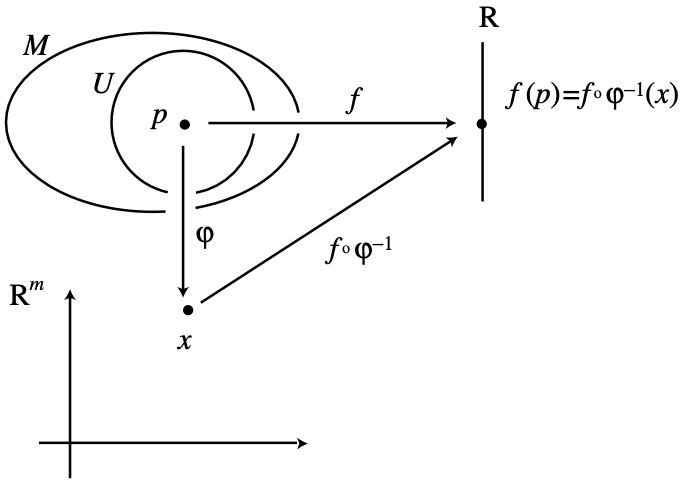
\includegraphics[width=\textwidth]{Images/function.png}
		\caption{A function $f\colon \M \to \R$ and its coordinate representation $f \circ \phi^{-1}$.}
		\label{fig:function}
	\end{subfigure}
	\caption{Curves and functions on a manifold.}
\end{figure}

%***************** VECTORS ********************
\subsection{Vectors}
A useful way to define a \emph{vector} on a manifold is through directional derivatives of functions along curves. Let $c\colon (a,b) \to \M$ be a curve with $c(0)=p$, and let $f \colon \M \to \R$ be any smooth function, as showed in fig.~\ref{fig:vector}. The \emph{tangent vector} at $p$ is the directional derivative of $f(c(t))$ along the curve $c(t)$ at $t=0$, that is,
\begin{equation}
	X[f] \coloneq \left. \frac{\ud f (c(t))}{\ud t}\right|_{t=0} = \left. \frac{\partial f}{\partial x^\mu} \frac{\ud x^\mu(c(t))}{\ud t} \right|_{t=0} = X^\mu \left(\frac{\de f}{\de x^\mu}\right),
\end{equation}
where we defined
\begin{equation}\label{eq:def-vectors}
	X = X^\mu \left(\frac{\de}{\de x^\mu}\right), \quad X^\mu = \left. \frac{\ud x^\mu(c(t))}{\ud t} \right|_{t=0} .
\end{equation}

\begin{figure}
	\centering
	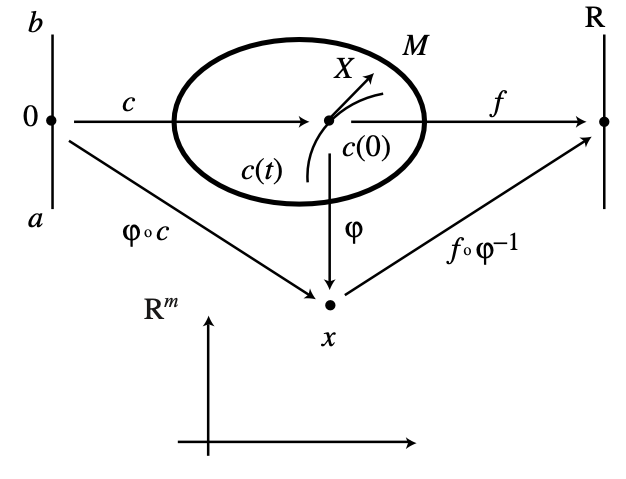
\includegraphics[width=0.5\textwidth]{Images/vector.png}
	\caption{A curve $c$ and a function $f$ define a tangent vector along the curve in terms of directional derivatives.}
	\label{fig:vector}
\end{figure}

Two curves $c_1(t)$ and $c_2(t)$ define the \emph{same} tangent vector at $p$ if
\begin{equation}
	c_1(0)= c_2(0)=p
\end{equation}
and
\begin{equation}
	\left. \frac{\ud x^\mu(c_1(t))}{\ud t} \right|_{t=0} = \left. \frac{\ud x^\mu(c_2(t))}{\ud t} \right|_{t=0} .
\end{equation}

The above relation defines an \emph{equivalence class}, and a vector $X$ at $p\in\M$ is an equivalence class of curves, that is,

\begin{equation}
	[c(t)] = \left\{ \tilde{c}(t) \; \Big| \; \tilde{c}(0) = c(0) \; \textit{and} \; \left. \frac{\ud x^\mu (\tilde{c}(t))}{\ud t}\right|_{t=0} = \left. \frac{\ud x^\mu (c(t))}{\ud t}\right|_{t=0} \right\} .
\end{equation}

The space of all such vectors at $p$ is the \emph{tangent space} $T_p \M$. A basis for $T_p \M$ is given by
\begin{equation}
	\left\{ e_\mu = \frac{\de}{\de x^\mu} \right\}   , \quad \mu = 1, \dots, n,
\end{equation}
making $\dim T_p \M = \dim \M = n$. Further, for each $V \in T_p \M$, we can expand it as $V = V^\mu e_\mu = V^\mu \de_\mu$, and we call $V^\mu$ the components of $V$ with respect to the basis.

%***************** ONE-FORMS ********************
\subsection{One-Forms}
Since each $T_p \M$ is a vector space, its \emph{dual} space $T^*_p \M$, called the \emph{cotangent space}, consists of linear functionals on $T_p \M$. An element 
\begin{equation}
    T^*_p \M \ni \omega \colon T_p \M \to \R
\end{equation}
is called \emph{one-form} at $p$. The simplest example is the \emph{differential} $\ud f$ of a function $f \in \F(\M)$. Its action on a vector $V \in T_p \M$ is given by
\begin{equation}
	\scalar{\ud f}{V} \equiv V[f] = V^\mu \frac{\de f}{\de x^\mu} \in \R.
\end{equation}

In coordinates $x = \phi(p)$, it can be expanded as
\begin{equation}
	\ud f = \frac{\de f}{\de x^\mu} \ud x^\mu,
\end{equation}
which clearly shows that $\{ \ud x^\mu \}$ is a basis of $T^*_p \M$, dual to $\{ \de_\mu \}$, since
\begin{equation}
	\scalar{\ud x^\mu}{\de_\mu} = \frac{\de x^\nu}{\de x^\mu} = \delta^\nu_\mu .
\end{equation}

For a generic one-form $\omega \in T^*_p \M$ and a generic vector $V \in T_p \M$, the \emph{inner product}
\begin{equation}
    \scalar{.}{.}\colon T^*_p \M \times T_p \M \to \R
\end{equation}
is defined by
\begin{equation}\label{eq:def-inner-product-vector-one-form}
	\scalar{\omega}{V} = \omega_\mu V^\mu \scalar{\ud x^\mu}{\de_\nu} = \omega_\mu V^\nu \delta^\mu_\nu = \omega_\mu V^\mu.
\end{equation}

%***************** TENSORS AND TENSOR FIELDS ********************
\subsection{Tensors and Tensor Fields}
In multilinear algebra, a \emph{tensor} of type $(q,r)$ at $p \in \M$ is a multilinear map 
\begin{equation}
	T^{(q,r)} \colon
	\underbrace{T^*_p \M \otimes \dots \otimes T^*_p \M}_\text{$q$ times}
	\otimes
	\underbrace{T_p \M \otimes \dots \otimes T_p \M}_\text{$r$ times} \longrightarrow \R.
\end{equation}

In coordinates, picking dual basis, such a tensor can be expanded as
\begin{equation}
	T^{(q,r)} = \tensor{T}{^{\mu_1}^\dots^{\mu_q}_{\nu_1}_\dots_{\nu_r}} \frac{\de}{\de x^{\mu_1}} \dots \frac{\de}{\de x^{\mu_q}} \ud x^{\nu_1} \dots \ud x^{\nu_r}.
\end{equation}

The set of type $(q,r)$ tensors at $p \in \M$ is denoted by $\Tau^q_{r;p}(\M)$. A vector is a $(1,0)$ tensor, while a one-form is a $(0,1)$ tensor.

In order to probe a manifold's structure, it's necessary to introduce fields, which are smooth objects defined for each point of $\M$. Knowing the tensor structure at a point, it's easy to generalize it to the entire manifold.

Considering as an example a $(1,0)$ tensor, a \emph{vector field} is a vector assigned smoothly to each point of $\M$. In other words, $V$ is a vector field if $V[f] \in \F(\M)$, for any $f \in \F(\M)$. Hence, each component of a vector field is itself a smooth function from $\M$ to $\R$. We denote the set of vector fields with $\X(\M)$. Then, a vector $X \in \X(\M)$ computed at a point $p \in \M$ is a vector at $T_p \M$, meaning $X|_p \in T_p \M$.

Taking two vector fields $X,Y \in \X(\M)$, the \emph{Lie bracket}, or \emph{commutator}, $[X,Y]$ is another vector field, which acts on a generic function $f \in \F(\M)$ by
\begin{equation}
	[X,Y](f) = X (Y[f]) - Y(X[f]).
\end{equation}

Generalizing, a \emph{tensor field} of type $(q,r)$ is a smooth assignment of an element of $\Tau^q_{r;p}(\M)$ at each point $p \in \M$. The set of tensor fields of type $(q,r)$ on $\M$ is denoted by $\Tau^q_r(\M)$.

%***************** FLOW BY VECTOR FIELD ********************
\subsection{Flow generated by a vector field}
A smooth vector field on a manifold naturally gives rise to a flow, a continuous mapping that describes how points move along the trajectories defined by the field.

Specifically, if $X$ is a vector field on $\M$, its associated flow is given by the map
\begin{equation}
    \sigma \colon \R \times \M \to \M,
\end{equation}
such that for each point $x$ in $\M$, the curve defined by $t \mapsto \sigma(t, x)$ is an integral curve of $X$. In other words, at each parameter value $t$ the tangent vector to the curve coincides with the value of $X$ at the point $\sigma(t,x)$.

In local coordinates, if we write $X$ in the form
\begin{equation}
    X = X^\mu \de_\mu,
\end{equation}
then the integral curve passing through an initial point $x_0$ satisfies the system of ordinary differential equations
\begin{equation}\label{eq:ode-flow-coordinates}
	\frac{\ud}{\ud t} \sigma^\mu (t,x_0) = X^\mu (\sigma(t,x_0)),
\end{equation}
with the initial condition
\begin{equation}\label{eq:ode-flow-initial-condition}
	\sigma^\mu(0,x_0) = x^\mu_0.
\end{equation}

A key property of the flow is its group-like behaviour. Indeed, for any two real numbers $t$ and $s$ and for any $x\in\M$, we have
\begin{equation}\label{eq:property-flow}
	\sigma(t, \sigma^\mu(s,x)) = \sigma(t+s,x),
\end{equation}

This property states that flowing first for a parameter $s$ and then for an additional parameter $t$ is equivalent to flowing continuously for a parameter $t + s$. It also implies that each mapping $\sigma(t,\,\cdot)$ is invertible with inverse $\sigma(-t,\,\cdot)$.

Applying the existence and uniqueness theorems for ordinary differential equations, one can prove the following theorem.

\begin{theorem}[Fundamental Existence Theorem for Flows]
	For any point $x \in \M$, there exists a unique differentiable map $\sigma \colon \R \times \M \to \M$, satisfying
	\begin{itemize}
		\item $\sigma(0,x) = x$;
		\item $t \mapsto \sigma(t,x)$ is a solution of~\eqref{eq:ode-flow-coordinates} and~\eqref{eq:ode-flow-initial-condition};
		\item $\sigma(t,\sigma^\mu(s,x)) = \sigma(t+s,x)$.
	\end{itemize}
\end{theorem}

It is important to note that if the vector field $X$ is complete — that is, if every integral curve can be extended for all values of the parameter — then the flow is globally defined on $\R$. In contrast, if $X$ is not complete, the flow might only exist around $t = 0$.

Just as flows generated by vector fields encode the dynamics of points on a manifold, the Ricci flow encodes the information about the evolution of a manifold's metric. The correct setting to work in is a Riemannian manifold. 


%***************** RIEMANNIAN MANIFOLDS ********************
\subsection{Riemannian Manifolds}
A Riemannian manifold is a smooth manifold equipped with a Riemannian metric~\cite{lee:riemann}.

\begin{definition}
	Let $\M$ be a differentiable manifold. A \emph{Riemannian metric} $g$ on $\M$ is a type $(0,2)$ tensor field on $\M$ such that, at each point $p \in \M$:
	\begin{itemize}
		\item $g_p (U,V) = g_p (V,U)$,
		\item $g_p(U,V) \geq 0$, where the equality holds only when $U=0$.
	\end{itemize}
	Here, $U,V \in T_p \M$ and $g_p = g|_p$. Basically, $g_p$ is a symmetric positive-definite bilinear form.
\end{definition}

Recall the previous definition of inner product~\eqref{eq:def-inner-product-vector-one-form} between vectors and dual forms. For $V \in T_p \M$ and $\omega \in T^*_p \M$, the inner product is given by $\scalar{.}{.} \colon T^*_p \M \times T_p \M \to \R$. If there exists a metric tensor $g$, then, we can use it to define the inner product between two vectors $U,V \in T_p \M$, specifically by $g_p(U,V)$. Since $g_p \colon T_p \M \otimes T_p \M \to \R$, we may define a linear map $g_p(U,.) \colon T_p \M \to \R$ by $V \mapsto g_p(U,V)$. Then, it's straightforward that $g_p(U,.) \in T^*_p \M$ is a one-form. Thus, the metric $g_p$ gives rise to an isomorphism between $T_p \M$ and $T^*_p \M$.

Choosing a chart $(\phi,U)$, with coordinates $\{ x^\mu \}$, we can express the metric tensor in local coordinates as
\begin{equation}
	g_p = g_{\mu\nu}(p) \ud x^\mu \otimes \ud x^\nu, \quad g_{\mu\nu}(p) = g_p (\de_\mu, \de_\nu) = g_{\nu\mu}(p), \quad p \in \M.
\end{equation}

It is usual convention to omit the point $p$, denote the inverse metric as $g^{\mu\nu}$, and the determinant as $\det(g_{\mu\nu}) \coloneq g$ and $\det(g^{\mu\nu}) \coloneq g^{-1}$. Thus, the isomorphism between $T_p \M$ and $T^*_p \M$ can be expressed as
\begin{equation}
	\omega_\mu = g_{\mu\nu} U^\nu, \quad U^\mu = g^{\mu\nu} \omega_\nu .
\end{equation}
One implicitly refers to this isomorphism by saying that the metric allows raising and lowering indices.

In a Riemannian manifold, the standard notion of differentiation does not preserve the tensorial character of geometric objects. To overcome this difficulty, we introduce the concept of the \emph{covariant derivative}. It extends the idea of directional derivatives to curved spaces, and allows us to define the concept of parallelism on a manifold.

%***************** COVARIANT DERIVATIVE ********************
\subsection{Covariant Derivatives}
We first introduce the concept of an \emph{affine connection}.
\begin{definition}
    An \emph{affine connection} $\nabla$ is a map $\nabla \colon \X(\M) \times \X(\M) \to \X(\M)$, or $(X,Y) \mapsto \nabla_X Y$ which satisfies the following conditions
    \begin{subequations}
        \begin{align}
            \nabla_X (Y + Z) &= \nabla_X Y + \nabla_X Z \\
            \nabla_{(X+Y)} Z &= \nabla_X Z + \nabla_Y Z \\
            \nabla_{(fX)} Y &= f \nabla_X Y \\
            \nabla_X (fY) &= X[f] Y + f \nabla_X Y,
        \end{align}
    \end{subequations}
    where $f \in \F(\M)$ and $X,Y,Z \in \X(\M)$.
\end{definition}

Take a chart $(U, \phi)$ with the coordinate $x = \phi(p)$ on $\M$, and define the functions $\Gamma^\lambda_{\nu\mu}$, called \emph{Christoffel symbols}, by
\begin{equation}
    \nabla_\nu e_\mu \equiv \nabla_{e_\nu} e_\mu = e_\lambda \Gamma^\lambda_{\nu\mu},
\end{equation}
where $\{e_\mu\} = \{\de_\mu\}$ is the coordinate basis in $T_p \M$. By computing their transformation rule under a generic change of coordinates, one can show that Christoffel symbols are \emph{not} components of a tensor.

Once the action of $\nabla$ on the basis vectors is defined, we can compute its action on any vector, i.e.,
\begin{equation}\label{eq:def-cov-der}
    \nabla_V W = V^\mu \left( \frac{\de W^\lambda}{\de x^\mu} + W^\nu \Gamma^\lambda_{\mu\nu} \right) e_\lambda .
\end{equation}

In particular, $\nabla$ maps two vectors $V$ and $W$ to a new vector given by the right-hand side of eq.~\eqref{eq:def-cov-der}, whose $\lambda$th component is $V^\mu \nabla_\mu W^\lambda$, where
\begin{equation}
    \nabla_\mu W^\lambda \equiv \frac{\de W^\lambda}{\de x^\mu} + \Gamma^\lambda_{\mu\nu} W^\nu
\end{equation}

Beyond vector fields, the concept of the covariant derivative extends naturally to tensor fields of any rank. For a general tensor field $T$ of type $(q, r)$, the covariant derivative $\nabla T$ is defined to behave as a tensor of type $(q, r+1)$ and to satisfy the appropriate product rule with respect to the tensor contractions and tensor products.

For Riemannian manifolds endowed with a metric tensor $g$, the affine connection can be chosen to be \emph{compatible} with the metric, meaning that
\begin{equation}
    \nabla_X g = 0, \quad \forall X \in \X(\M).
\end{equation}
Intuitively, this means that angles between vectors are conserved while parallelly transporting them along each other.

Curvature provides a quantitative measure of how a manifold deviates from being flat. Since $\Gamma$ is not a tensor, it can't have an intrinsic geometric meaning as a measure of the curvature. To serve this purpose, one introduces the \emph{torsion} and \emph{Riemann tensor}.

%***************** CURVATURE ********************
\subsection{Curvature and Ricci Tensor}

The \emph{torsion tensor} $T \colon \X(\M) \otimes \X(\M) \to \X(\M) $ and the \emph{Riemann tensor} $R \colon \X(\M) \otimes \X(\M) \otimes \X(\M) \to \X(\M) $, also called \emph{curvature tensor}, are defined by
\begin{align}
    T(X, Y) &\equiv \nabla_X Y - \nabla_Y X - [X,Y], \\
    R(X,Y,Z) &\equiv \nabla_X \nabla_Y Z - \nabla_Y \nabla_X Z - \nabla_{[X,Y]} Z \label{eq:def-riemann}.
\end{align}

For simplicity, we consider torsionless connections, for which the Christoffel symbols are symmetric, meaning that
\begin{equation}
    \Gamma^\lambda_{\nu\mu} = \Gamma^\lambda_{\mu\nu} .
\end{equation}

Further, for a metric compatible connection, one can derive the following expression
\begin{equation}
    \Gamma^\lambda_{\mu\nu} = \frac{1}{2} g^{\lambda\rho} \left( \de_\nu g_{\mu\rho} + \de_\mu g_{\nu\rho} - \de_\rho g_{\mu\nu} \right),
\end{equation}
and the Riemann tensor has components
\begin{equation}
    R_{\mu\nu\rho\sigma} = \frac{1}{2} \left( {\de}^2_{\nu\rho} g_{\mu\sigma} - {\de}^2_{\nu\sigma} g_{\mu\rho} + {\de}^2_{\mu\sigma} g_{\nu\rho} - {\de}^2_{\mu\rho} g_{\nu\sigma} \right) .
\end{equation}

Using the general definition~\eqref{eq:def-riemann}, one can prove the following identities
\begin{subequations}
\begin{gather}
    R_{\mu\nu\rho\sigma} = - R_{\nu\mu\rho\sigma} = - R_{\mu\nu\sigma\rho}, \\
    R_{\mu\nu\rho\sigma} = R_{\rho\sigma\mu\nu}, \\
    R^\mu_{\nu\rho\sigma} + R^\mu_{\sigma\nu\rho} + R^\mu_{\rho\sigma\nu} = 0.
\end{gather}
\end{subequations}

The symmetries allow us to define the symmetric tensor $R_{\mu\nu} = R^\lambda_{\mu\lambda\nu}$, called \emph{Ricci tensor}, and the \emph{Ricci scalar} $R = R^\mu_\mu$.